\section{Driver Applications}
\label{sec:apps}

\FIXME{RC: The text below is mostly from~\cite{cag18}.}

\subsection{Real-Time Hybrid Simulation of Civil Structures}

Our first cyber-physical application example comes from the domain of
\emph{real-time hybrid structural} (RTHS)~\cite{RTHS} experiments used in
structural and earthquake engineering.  In these experiments, a physical
specimen is connected to a low-level control loop via sensors
that can measure the position and/or acceleration of the specimen continuously,
communicate those measurements frequently as digital readings through a DAQ
board, and in turn receive and apply commands sent by the low-level
controller through the DAQ board to actuators that are also connected to
the specimen.  Low-level control design includes both the dynamics of
the specimen and compensation for the dynamics of
the actuators to ensure that appropriate forces are applied to the specimen
over time. The sensor measurements are used as inputs to a simulation
(e.g., using a finite element model) that computes the behavior of the overall structure,
including the next set of forces to apply to the specimen at the next time step.  Within
each iteration, both the low-level control loop and the simulation must complete within a
millisecond or less to avoid losing high-frequency vibrations or other behaviors
of the specimen.

Figure~\ref{fig:rths} shows a scale-model version of such an experiment, at
Washington University in St. Louis.  Full-scale experiments require hydraulic
actuators and other capabilities found in facilities such as the Bowen Laboratory
at Purdue University, and our experiences working with both versions has shown
that scale-model experiments offer a useful setting for designing, developing, and
debugging cyber-physical experiments before moving them to the full-scale setting.
\FIXME{RC: add picture of full-scale system at Purdue.}

\begin{figure}[ht]
\centering
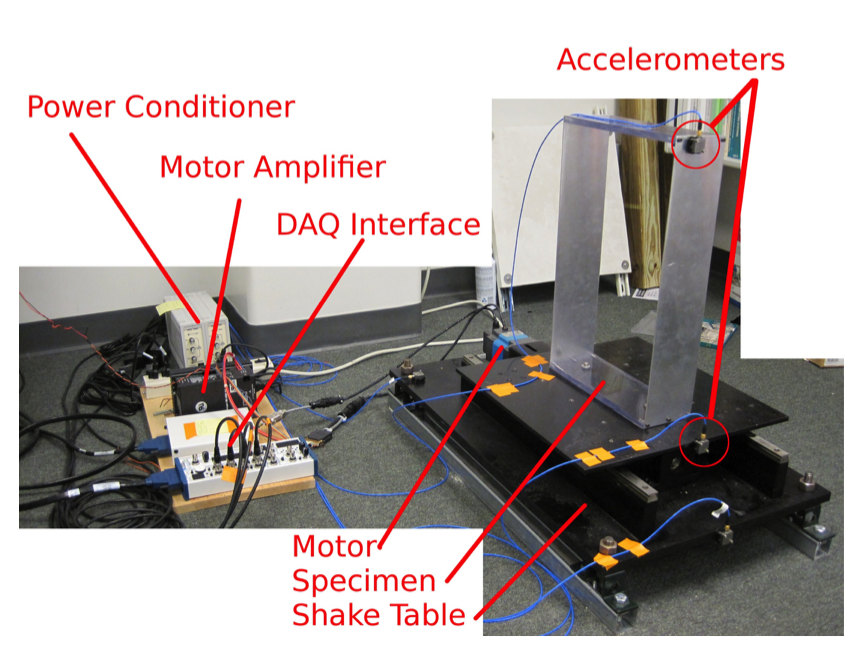
\includegraphics[width=0.5\columnwidth]{rths}
\caption{RTHS experiment at Washington University in St. Louis.}
\label{fig:rths}
\end{figure}

Higher-level objectives include the ability to substitute simulated versus physical versions
of different parts of a structure~\cite{Huang10}, and through advances in
parallel real-time concurrency platforms to trade-off computational demand and
time scales~\cite{Ferry14} allowing resources to be concentrated for portions of
the structure that are most significant.

\FIXME{RC: we need to let the reader know that this is a finite-element model, and
point out that \emph{lots} of other applications use finite-element models of some
aspect of the physical world.}

\FIXME{RC: tie this into the research questions we address later.}

\subsection{Catoptric Systems}

Figure~\ref{fig:amp} shows a prototype catoptric (mirror) surface
called \emph{AMP} that was
designed, fabricated, and installed during an undergraduate architecture studio
taught by Co-PI C.~Ahrens. The installation redirects light from gable ends of an
existing building into the darker recesses of the atrium
to create better natural lighting where it is desired.
We next developed a
new version in which over 600 mirrors are under
active, 2-axis control and therefore the mirrors
can be pointed in different directions dynamically as desired over
time~\cite{acmbg19,acmb18,cagm18}.
This next-generation installation is within
the south wall of the Steinberg Hall atrium on the campus of
Washington University; a subset of the mirrors in this new
installation is shown in Figure~\ref{fig:steinberg}.

\begin{figure}[ht]
\centering
\subfloat[\mbox{ }]{
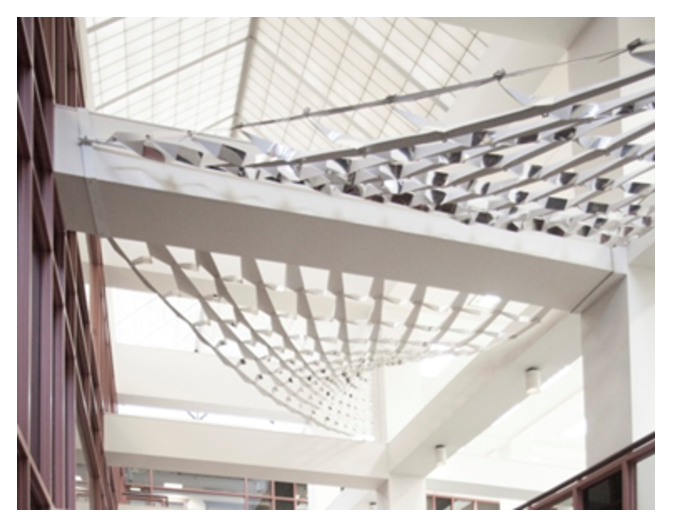
\includegraphics[width=0.43\linewidth]{amp}
\label{fig:amp}}
\quad %\qquad
\subfloat[\mbox{ }]{
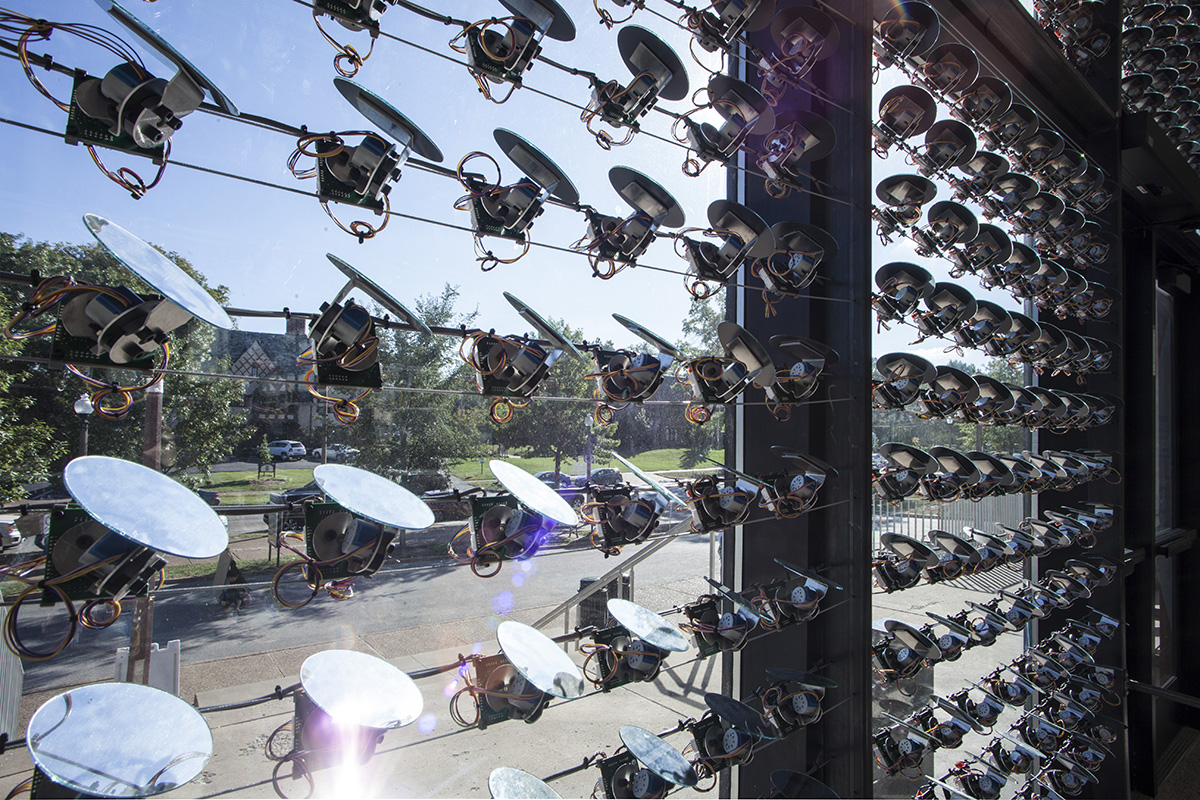
\includegraphics[width=0.5\linewidth]{CS_prototype_012_sm}
\label{fig:steinberg}}
\caption{Catoptric system prototypes.
(a)~\emph{AMP}, TRex building, St.~Louis.
(b)~Steinberg Hall, St.~Louis.
}
\label{fig:proto}
\end{figure}


Using ray tracing algorithms and straightforward low-level control mechanisms,
we can position a set of mirrors to direct light where it is desired. The
high-level decisions revolve around the questions of, ``how do we operate
the system safely?'' and, ``where do we want the light to be?''
The first question relies on feedback obout the actual configuration of the system.
One feedback mechanism we will use is visual data (imagery and video). This
will include determination of the true orientation of each mirror, providing information
on the available light and its current positioning, as well well as providing feedback
on benefits accrued.

The second question becomes even more interesting if we expand the
higher level options to include varying the intensity of daylight that is
directed into an area according to the area's use (e.g., lower to improve
contrast when computer screens are being used, or higher when people are
reading paper materials), or the ability to direct incoming sunlight that
is not needed for another purpose into a heat exchanger that can harvest
energy for the building's HVAC system.  Given a bounded resource
(currently available sunlight), we now are charged
with balancing the relative benefits of natural sunlight illumination within
a physical space vs.~the harvesting of thermal energy which can potentially
reduce operating costs for that same physical space.

Data are streaming from the sensors providing feedback, as well as the users'
directions for use of the available light.  Especially for safety concerns, the
latency constraints for processing this data stream and making decisions are
strict.  Also, for the Steinberg prototype, several of the communications
between computational elements are via wireless links.  Neither best effort computation
nor communication will be sufficient. Guarantess are needed.
